\documentclass[9pt,twocolumn,twoside]{../../styles/osajnl}
\usepackage{fancyvrb} \journal{i524}

\title{Detecting Stop Signs in Images and Videos in a Robot Swarm}

\author[1,*]{Rahul Raghatate}
\author[1]{Snehal Chemburkar}

\affil[1]{School of Informatics and Computing, Bloomington, IN 47408,
  U.S.A.}

\affil[*]{Corresponding authors: rraghata@iu.edu, snehchem@iu.edu}

\dates{S17-IR-P003, \today}

\ociscodes{Street Signs, Ansible, Video Streams, OpenCV, Spark, Cloud}


\doi{\url{https://github.com/cloudmesh/sp17-i524/raw/master/project/S17-IR-P003/report/report.pdf}}

\begin{abstract}
This project is designed to deploy a scalable stop sign detection
algorithm to process real-time image and video streams. The deployment
is automated allowing for minimal user-interaction. Spark on Yarn
provides the distributed computing power required to scale the stop
sign detection algorithm to process big data. This system is useful in
automated driving vehicles and advanced driver assisted systems (ADAS)
to detect and classify the street signs and control the vehicle
accordingly. A comparative benchmark is developed based on the
performance of the application on multiple cloud systems.\newline
\end{abstract}

\setboolean{displaycopyright}{true}

\begin{document}

\maketitle

\section{Introduction}
There are many applications developed based on simple idea of object
detection, like auto-tagging pictures (e.g. Facebook, Phototime),
counting the number of people in a street (e.g. Placemeter), tracking
an object in video streams, detecting vehicles to name a few.  Based
on this concept of object detection, we deploy a scalable software for
stop sign detection using Spark on multiple clouds.  The software
deployment is automated using Ansible. Cloudmesh provides simple
command line interface for defining the number of clusters as well as
deploying them. Benchmarks are developed based on the performance of
this software on different cloud systems. The database of street signs
will be restricted to US street signs. The only publicly available
dataset for US traffic signs is the LISA dataset
\cite{paper-lisadataset} which is very huge. Hence, the video streams
used for this project are captured by us using a mobile camera.

OpenCV is a computer vision library used to process video streams in
Python. A lot of computing power goes into processing videos in
real-time, this is where the cloud systems come in. We leverage the
distributed computing power of Spark on Yarn for faster processing of
images and videos. This solution is deployed on two different clouds
to benchmark their performance.  In this era of autonomous driving and
advanced driver assisted systems (ADAS), detection and classification
of traffic signs is a handy feature. Benchmarks have been created for
the traffic sign detection on the German and Belgium Traffic Sign
Datasets \cite{paper-trafficsign}.

\section{Requirement Analysis}
The following technologies are used throughout the project:
\begin{itemize}
\item Cloudmesh provides command line interface to connect and deploy
  clusters to different cloud systems.
\item Ansible is an agentless, automated software deployment tool.
\item Python - Programming language.
\item Spark - Distributed computing engine.
\item YARN - is the resource manager for Spark.

\item OpenCV - Image and video analysis for street sign detection
  using open source computer vision libraries.The OpenCV library
  provides several transformations that can be applied to images(apply
  filters, transformation), detect and recognize objects in images.
\end{itemize}


\section{Scope}

The initial project idea was to automate the deployment of street sign
detection algorithm over multiple cloud systems. As we proceeded
through the project, we realized that training of Haar Cascade
classifier is challenging. For a training dataset of 1000 samples the
training can go on for 3-4 days. It turned out to be an exhaustive
process. The resultant classifiers were unable to detect the specific
signs. The details of the OpenCV training process we followed are
given in the appendix. Due to difficulty training classifiers for
street signs, we had to reduce the scope of this project to detect
only stop signs using a pre-trained classifier available on Github
\cite{}. The stop sign detection is implemented for both images and
videos using Spark.


\begin{figure*}[h]\centering
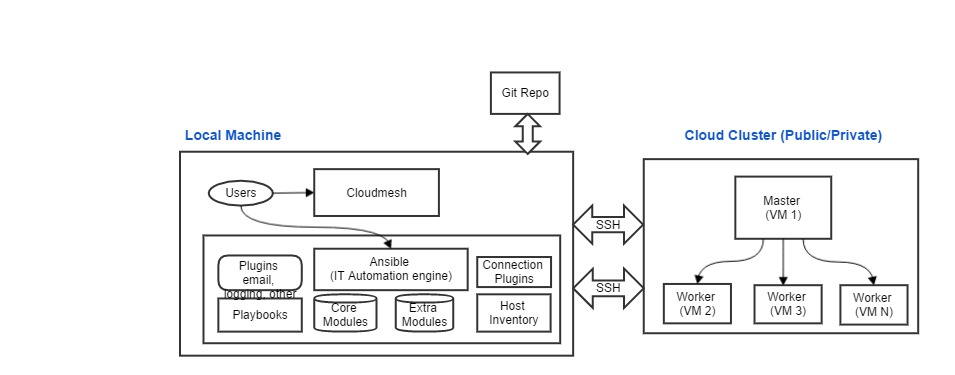
\includegraphics[width=\linewidth]{images/architecture}
\caption{System Architecture}
\label{fig:system}
\end{figure*}

\section{System Architecture}

Figure \ref{fig:system} shows an overview of our system
architecture. Ansible and Cloudmesh client are installed on the host
or local machine. Roles are defined in the Ansible playbook for each
of the different steps in the deployment process. We execute the
Ansible playbooks to instantiate the cloud machines, deploy Hadoop and
Spark on them and then carryout the stop sign detection on Spark using
Yarn resource manager. Once the job is submitted to Spark, the driver
program initializes the SparkContext object which is responsible for
the execution of the job. Input data is parallelized and sent to the
worker nodes for processing. Yarn acts as the resource manager and
provides executors to the worker nodes. The output is saved to the
local file system on the master node and transferred to the host
machine through a script. More details on the mechanics can be
understood in the following sections.

\section{Cloud Infrastructure}
For the purpose of this project, we have been provided with two clouds
– Chameleon \cite{www-chameleon} and Jetstream \cite{jetsream}
\cite{jetstream2}. Chameleon cloud is a National Science Foundation
funded experimental testbed that provides large scale cloud services
to "members of the US computer Science research community and its
international collaborators \cite{www-chameleon}." One can create
virtual machines and manage them through the OpenStack Horizon
interface. Jetstream allows researchers to leverage the computational
power of cloud while retaining the look and feel of our home
machines. Jetstream adds cloud based computational power to the
national cyberinfrastructure \cite{www-jetstream}. Both Chameleon and
Jetstream provide a cloud computing environment to researchers based
on OpenStack \cite{www-jetstream}. The comparison of hardware
specifications for the two cloud systems is given in table
\ref{tab:compare}.

\begin{table}[htbp]
\centering
\begin{tabular} {| c | c | c | }
\hline & Chameleon & Jetstream \\ [0.5ex] \hline CPU & Xeon X5550 &
Haswell E-2680 \\ \hline cores & 1008 & 7680 \\ \hline speed & 2.3GHz
& 2.5GHz\\ \hline RAM & 5376GB & 40TBr\\ \hline storage & 1.5PB & 2
TB\\ [1ex] \hline
\end{tabular}

\caption{\bf Comparison of Cloud Specification
  \cite{www-jetstream-cloud} \cite{www-chameleon-cloud}}
\label{tab:compare}
\end{table}

\section{Cloudmesh}
Cloudmesh provides an easy interface to multiple clouds such as
Chameleon and Jetstream through the command line. Cloudmesh client can
be installed via pip. It is a lightweight utility that enables users
to connect to different clouds from their laptops or computers. Users
can customize Cloudmesh client to suite their needs of
cyberinfrastructure. It provides simple command line scripts to deploy
Hadoop with Spark addon to either of the clouds mentioned in section
5.  A set of cluster machine instances can be defined using command:
\begin{verbatim} 
cm cluster define --count 3
\end{verbatim}

Cloudmesh commands to create and deploy Hadoop clusters with Spark are
included as tasks in the ansible playbooks to automate the deployment.

\section{Ansible Automation}
Ansible is an easy to use, opensource automation tool that is used to
automate the deployment of our project on the cloud
infrastructure. Ansible is an agentless tool, that is, it does not
require ansible to be deployed on the remote machines. It runs only on
the host machine to deploy the required processes to the remote
machines through SSH authentication.  Using Ansible, we can create
modules for each step of the deployment process and define the roles
individually. An inventory file is used to define the machines in
groups as required. A sample inventory file looks like:
\begin{verbatim} 
[master] 
192.128.0.1 
[workernode] 
192.168.0.2 
192.168.0.3
\end{verbatim}

Roles are defined in Ansible for the deployment of Hadoop-Spark
cluster, environment setup on the virtual machines, stop sign
detection as well as to fetch the results back to the local.

\section{Python-OpenCV}

Python is preferred due to ease of use and familiarity over other
programming languages. OpenCV also provides python library to enable
object detection in python using this computer vision library. The
initial scope included training a Haar Cascade Classifier to detect
traffic signs and then testing the classifier on test data. But as
explained in appendix section - Training a Haar Cascade Classifier - a
decent classifier could not be trained. The stop sign detection
algorithm utilizes a pre-trained stop sign classifier available on
Github to perform the detection in images and videos. The results of
the algorithm are saved as images in the
\texttt{\~/github/cloudmesh.street/ansible/output/output/} folder on
your local machine, assuming that the git repository is cloned to
\texttt{\~/github/cloudmesh.street/}. The output files will have a
bounding box around the detected object. The
signdetectionusingspark.py file is used to process both images and
videos. Based on whether the input is either image or video, the path
to these files has to be modified in the spark-submit task of ansible
playbook.

\section{Shell Script}
Shell script is used to time each of the deployment step for
benchmarking. Shell script is also useful in cases where a the
deployment terminates in an error and needs to be continued from some
intermediate steps. Individual shell scripts are created for each
tasks in case of such issues to allow execution from the point of
interruption.

\section{Benchmark}
Benchmarks are created based on the performance of the software in
different cloud environments. The benchmarks for Jetstream are limited
due to issues with their cloud. As the test data is images and videos,
spark ran into memory issues on the m1.small flavor. Hence, we have
done benchmakring using the medium and large flavours only. Tables
\ref{tab:jet} and \ref{tab:cham} reflect that the configurations for
the same flavors on the two clouds are different. We cannot directly
compare the performance if the two machines have different
specifications. Benchmarking is done for the deployment and the
analysis on Chameleon and Jetstream.

\begin{table}[htbp]
\centering
\begin{tabular} {| c | c | c | c |}
\hline JetStream & VCPU & RAM(GB) & Storage(GB)\\[0.5ex] \hline
m1.small & 2 & 4 & 20 \\ \hline m1.medium & 6 & 16 & 60 \\ \hline
m1.large & 10 & 30 & 60 \\[1ex] \hline
\end{tabular}

\caption{\bf Jetstream Flavour Specifications}
\label{tab:jet}
\end{table}

\begin{table}[htbp]
\centering
\begin{tabular} {| c | c | c | c |}
\hline Chameleon & VCPU & RAM(GB) & Storage(GB)\\[0.5ex] \hline
m1.small & 1 & 2 & 20 \\ \hline m1.medium & 2 & 4 & 40 \\ \hline
m1.large & 4 & 8 & 80 \\[1ex] \hline
\end{tabular}

\caption{\bf Chameleon Flavour Specifications}
\label{tab:cham}
\end{table}

\subsection{Chameleon Cloud Benchmarks}
\subsubsection{For flavor m1. medium and 50 Test Images}
Figure \ref{fig:cmed1} shows the time taken for analyzing the 50
images on Chameleon cloud for 1, 2, 3, 4, and 6 node clusters. We can
see that as the number of nodes increases the time taken to analyze
the images reduces. Figure \ref{fig:cmed2} reflects the total time
required to complete the deployment. We can see that the total
deployment time doesn't vary much upto 4 nodes but there is a steep
increase in the deployment time for 6 node cluster.
\begin{figure}[htbp]
\centering
\fbox{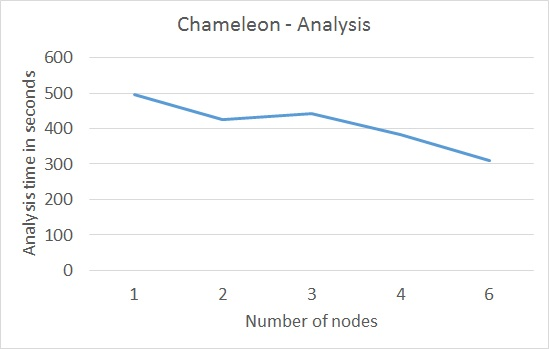
\includegraphics[width=\linewidth]{images/cham50.jpg}}
\caption{Time taken by sign detection task - 50 test images}
\label{fig:cmed1}
\end{figure}

\begin{figure}[htbp]
\centering
\fbox{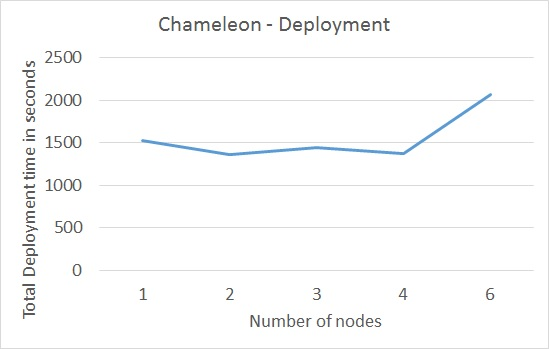
\includegraphics[width=\linewidth]{images/cham50_dep.jpg}}
\caption{Time taken for complete deployment - 50 test images}
\label{fig:cmed2}
\end{figure}

\subsubsection{For flavor m1.medium and a Video Input }
The video input file tested on the medium flavor is just 2 sec long
but since it gets converted to frames, it comes out to 53 images that
are sent to spark for processing.  Figure \ref{fig:cmed4} shows the
time taken for analyzing a single video that is 2 seconds long on
Chameleon cloud for 3, 4, 6, and 7 node clusters. We can see that as
the number of nodes increases the time taken to analyze the images
reduces a lot. Figure \ref{fig:cmed3} reflects the total time required
to complete the deployment. We can see that the total deployment time
doesn't vary much upto 4 nodes but there is a steep increase in the
deployment time for 6 node cluster.

\subsubsection{For flavor m1.large and a Video Input }
The video input file tested on large flavor is 5 sec long and after
extracting the frames, it comes out to 120 images that are sent to
spark for processing.
Figure \ref{fig:cmed6} shows the time taken for analyzing a single
video that is 5 seconds long on Chameleon cloud for 1, 2, 3, and 4
node clusters. We can see that as the number of nodes increases the
time taken to analyze the reduces which is expected. Figure
\ref{fig:cmed5} reflects the total time required to complete the
deployment. We can see that the total deployment time increases
steeply at first and then starts to normalize.

\begin{figure}[htbp]
\centering
\fbox{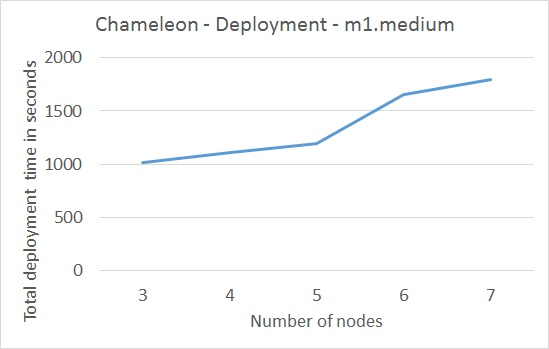
\includegraphics[width=\linewidth]{images/chamvid_dep_m.jpg}}
\caption{Time taken for complete deployment - 1 Video (2 sec)}
\label{fig:cmed3}
\end{figure}


\begin{figure}[htbp]
\centering
\fbox{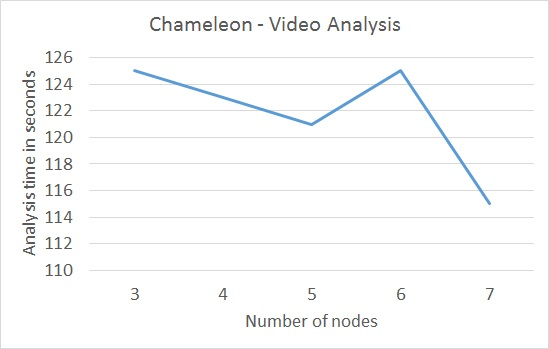
\includegraphics[width=\linewidth]{images/chamvid_ana.jpg}}
\caption{Time taken for sign detection task - 1 Video (2 sec)}
\label{fig:cmed4}
\end{figure}

\begin{figure}[htbp]
\centering
\fbox{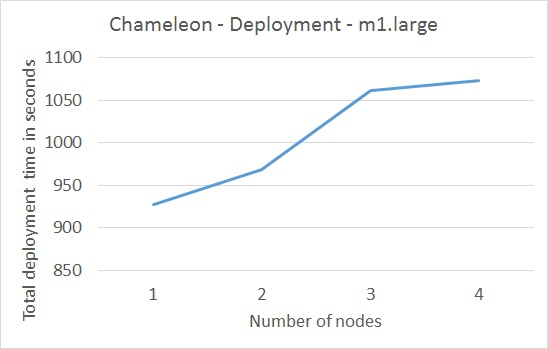
\includegraphics[width=\linewidth]{images/chamvid_dep_l.jpg}}
\caption{Time taken for complete deployment - 1 Video (5 sec)}
\label{fig:cmed5}
\end{figure}




\begin{figure}[htbp]
\centering
\fbox{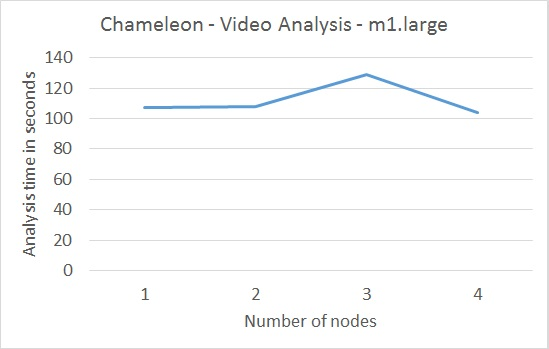
\includegraphics[width=\linewidth]{images/chamvid_ana_l.jpg}}
\caption{Time taken for sign detection task - 1 Video (5 sec)}
\label{fig:cmed6}
\end{figure}

\subsection{Jetstream Cloud Benchmarks}

\ref{fig:jmedium4} shows the time taken to the complete deployment on
Jetstream when the number of images parsed are 4. It can been seen
from the graph that as the number of nodes is increased the processing
time is reduced. \ref{fig:jmedium5} and \ref{fig:jmedium6} reflect the
performance of Jetstream cloud for 4 and 50 input images
respectively. Sufficient data could not be gathered for Jetstream due
to some issues with Jetstream. Hence we cannot conclude much about the
performance of Jetstream.

\begin{figure}[htbp]
\centering
\fbox{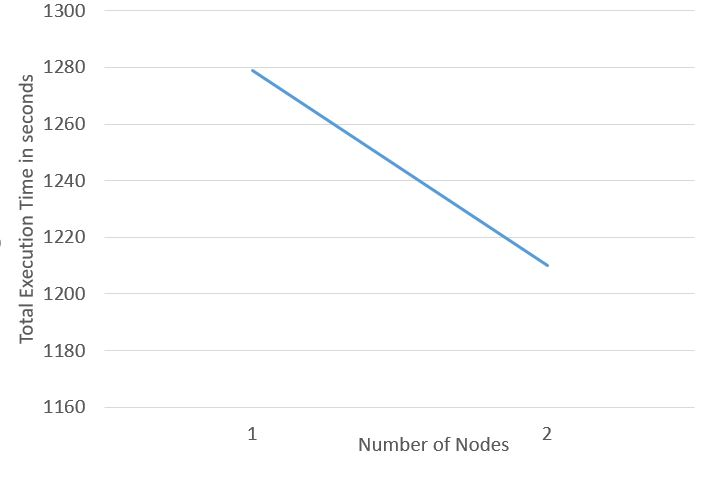
\includegraphics[width=\linewidth]{images/jetstream4.JPG}}
\caption{Total time required to deploy for 4 test images}
\label{fig:jmedium4}
\end{figure}

\begin{figure}[htbp]
\centering
\fbox{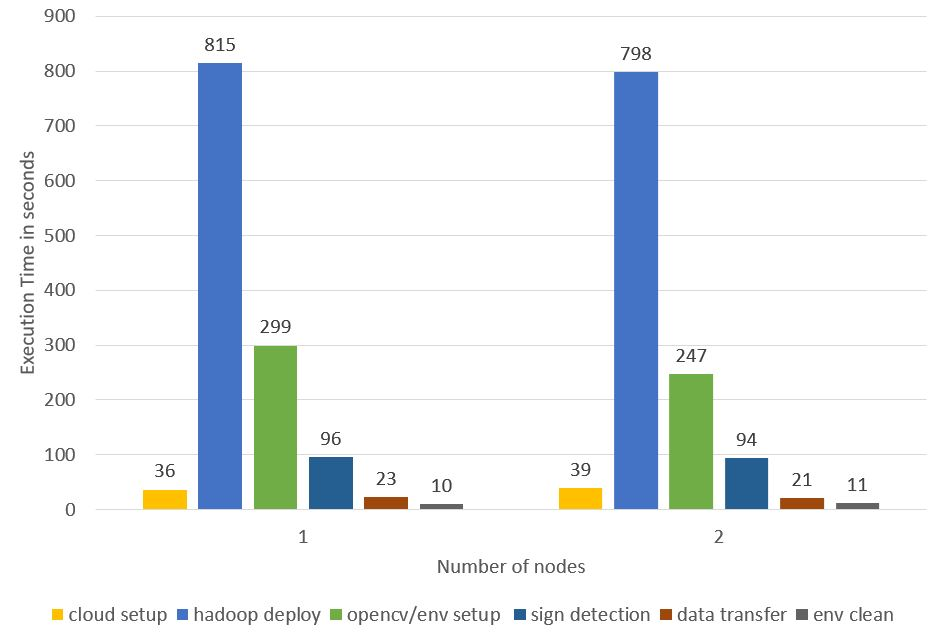
\includegraphics[width=\linewidth]{images/jmedium4.jpg}}
\caption{Time taken by each task for 4 test images}
\label{fig:jmedium5}
\end{figure}



\section{Use Cases}
\begin{enumerate}
\item Street Sign Detection for autonomous vehicles.
\item Analysis of traffic signs in Google Street View to estimate all
  signs ahead hence, useful in ambulance , fire brigade services,
  simplest path finder etc.
\end{enumerate}
\begin{figure}[htbp]
\centering
\fbox{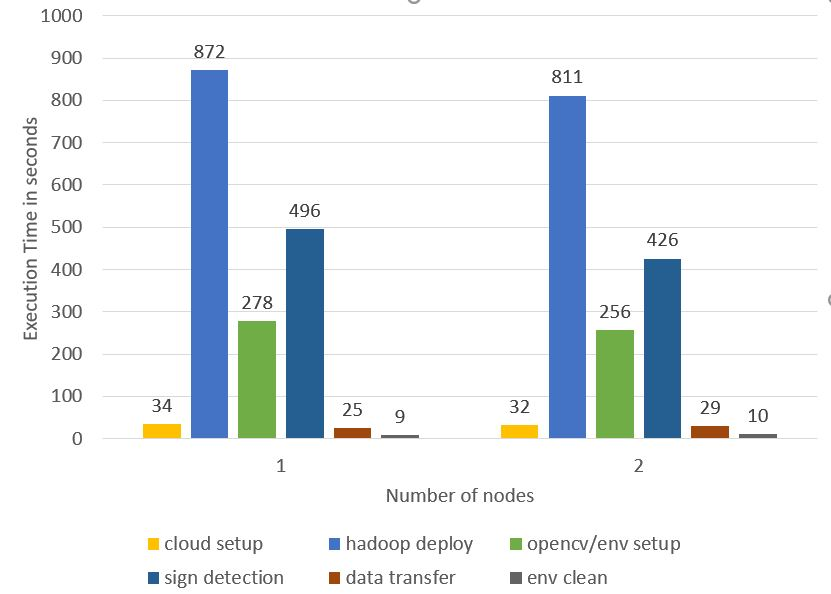
\includegraphics[width=\linewidth]{images/jmedium50.jpg}}
\caption{Time taken by each task for 50 test images}
\label{fig:jmedium6}
\end{figure}

\section{Future Work}
This work can be expanded to detect and classify all the U.S traffic
signs which can be adapted for advanced driver assisted systems (ADAS)
. Moreover, efficiency of sign detection over cloud can be increased
by effective distribution of data, for e.g using Hadoop distributed
file system. An extension of the stop sign detection in video streams
would be to output the data as videos rather than images in
realtime. As the current system is scalable, benchmarks can be
developed for larger dataset with multiple classifier, similar to the
German and Belgium Traffic Sign Detection and Classification
benchmarks \cite{paper-trafficsign}.

\section{Conclusion}

We have been able to successfully deploy the software to Jetstream and
Chameleon clouds and test their performance. On large flavors of
chameleon cloud the deployment time starts to flatten out over the
curve.As the number of nodes increases the time taken to deploy Hadoop
and spark to those clusters increases and on the up side the analysis
on Spark is faster.

\section*{Acknowledgements}
This project is undertaken as part of the I524: Big Data and Open
Source Software Projects coursework at Indiana University. We would
like to thank Prof. Gregor von Laszewski, Prof. Gregory Fox and the
Associate Instructors for their help and support. Results presented in
this paper were obtained using the Chameleon testbed supported by the
National Science Foundation.

% Bibliography
\bibliography{references}

\section*{Author Biographies}
\begingroup \setlength\intextsep{0pt}
\begin{minipage}[t][3.2cm][t]{1.0\columnwidth}
% Adjust height [3.2cm] as required for separation of bio photos.
  \begin{wrapfigure}{L}{0.25\columnwidth}
    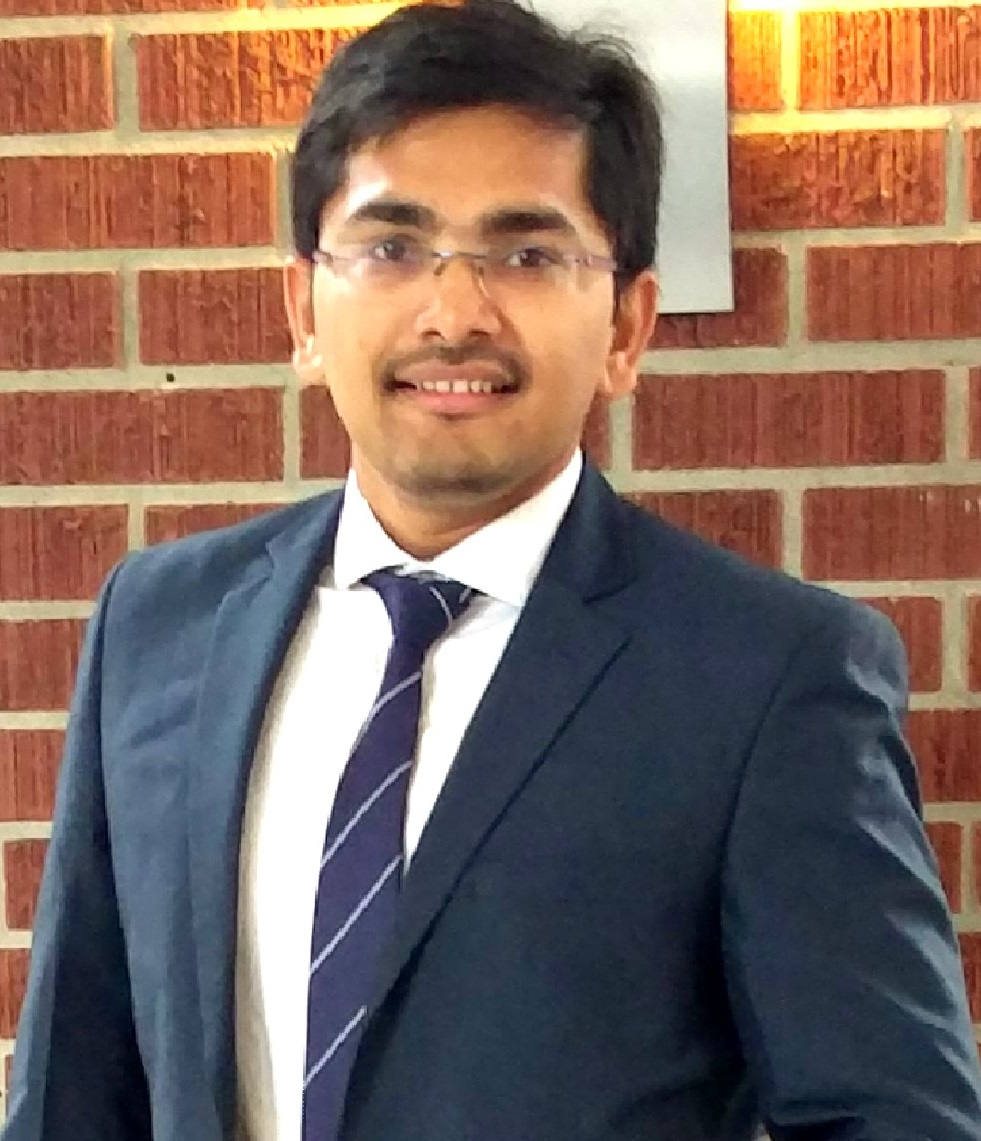
\includegraphics[width=0.25\columnwidth]{images/rahul_thumbnail.jpg}
  \end{wrapfigure}
  \noindent
  {\bfseries Rahul Raghatate} will receive his Masters (Data Science)
  in 2018 from The Indiana Univeristy Bloomington. His research
  interests include Big Data Technologies and Machine Learning.
\end{minipage}
\begin{minipage}[t][3.2cm][t]{1.0\columnwidth} % Adjust height [3.2cm] as required for separation of bio photos.
  \begin{wrapfigure}{L}{0.25\columnwidth}
    
\includegraphics[width=0.25\columnwidth]{images/alice_smith.eps}
  \end{wrapfigure}
  \noindent
  {\bfseries Snehal Chemburkar} is a graduate student at Indiana
  University. She will receive her degree in Data Science in 2018. Her
  research interests include Big Data and Machine Learning.
\end{minipage}
\endgroup \appendix

\section{OpenCV Image Processing}

OpenCV provides a range of computer vision algorithms to detect
objects in images. One of the simplest method for object detection is
based on color. The results of Color based detection method are
largely affected by the lighting conditions and one require the user
to calibrate multiple times before they might get a better result in
the real world \cite{paper-objectdetection}. Hence this technique is
not very popular when detecting objects in the real world Haar
features is a sophisticated technique that uses the features specific
to the object in question. It been seen that working with RGB pixel
values in every single pixel in the image results in computationally
expensive and slow feature calculation. “A Haar-like feature considers
neighboring rectangular regions at a specific location in a detection
window, sums up the pixel intensities in each region and calculates
the difference between these sums. This difference is then used to
categorize subsections of an image \cite{paper-objectdetection}.”
OpenCV provides a Haar feature based cascade classifier that can be
used for object detection, as proposed by in \cite{paper-ROD}.

\subsection{Data Collection}

The publicly available data set for U.S street signs is the LISA
traffic dataset \cite{paper-lisadataset}. This dataset contains images
for 47 different traffic signs. But since the data set itself is
approximately 7GB, we extracted 50 images from the dataset for the
purpose of testing. For our training set, we captured images of street
signs and put together a few positive images for the street signs. The
positive images were cropped to only contain the street sign and
resized to 50x50.

\subsection{Train a Haar feature-based Cascade Classifier}

Based on tutorials provided in \cite{www-coding-robin},
\cite{www-opencv} , we carried out multiple experiments to train a
classifier to detect street signs. Since each sign needed to trained
separately, we picked stop, yield, and signal ahead signs to start
with. To train a classifier, we firstly required gathering at least a
few positive and many negative images. The positive images are images
of the object alone cropped to a size of 24x24 or 50x50 whereas the
negative images should not contain the object in consideration
here. In case we have a single positive image or a few positive
images, OpenCV provides a utility called opencv\_createsamples to
generate the training and test datasets in *.vec format that is
supported by the opencv\_traincascade utility. The samples generated
from the opencv\_createsamples can be passed to the
opencv\_traincascade utility to get a trained classifier.  Multiple
experiments were carried out by differing the sample sizes (the width
by height of the positive images) and varying the number of positive
and negative images. As the dataset and width by height increases the
computational time increases. Below are the trainings that were
carried out for stop sign:

\begin{verbatim}
opencv_traincascade -data classifier -vec samples.vec 
-bg negatives.txt -numStages 20 -minHitRate 0.999 
-maxFalseAlarmRate 0.5 -numPos 120 -numNeg 200 -w 50 
-h 50 -mode ALL -precalcValBufSize 1024
-precalcIdxBufSize 1024
\end{verbatim}
\begin{verbatim}
opencv_traincascade -data classifier -vec samples.vec 
-bg negatives.txt -numStages 20 -minHitRate 0.999 
-maxFalseAlarmRate 0.5 -numPos 200 -numNeg 350 -w 50 
-h 50 -mode ALL -precalcValBufSize 1024
-precalcIdxBufSize 1024
\end{verbatim}
\begin{verbatim}
opencv_traincascade -data classifier -vec samples.vec 
-bg negatives.txt -numStages 20 -minHitRate 0.999 
-maxFalseAlarmRate 0.5 -numPos 600 -numNeg 100 -w 50 
-h 50 -mode ALL -precalcValBufSize 1024
-precalcIdxBufSize 1024
\end{verbatim}

When we increased the number of positive samples to 600 for the 50x50
image size, the training ran for 3.5 days. The resulting classifier
was unable to detect the stop signs in the test data. After a couple
more experiments and another week invested in training the classifier
to no good results, we found success with a pre-trained classifier for
stop signs available at \cite{github-stopsigns}. The results of this
classifier are shown in \ref{fig:detect}.

\begin{figure}[htbp]
\centering
\fbox{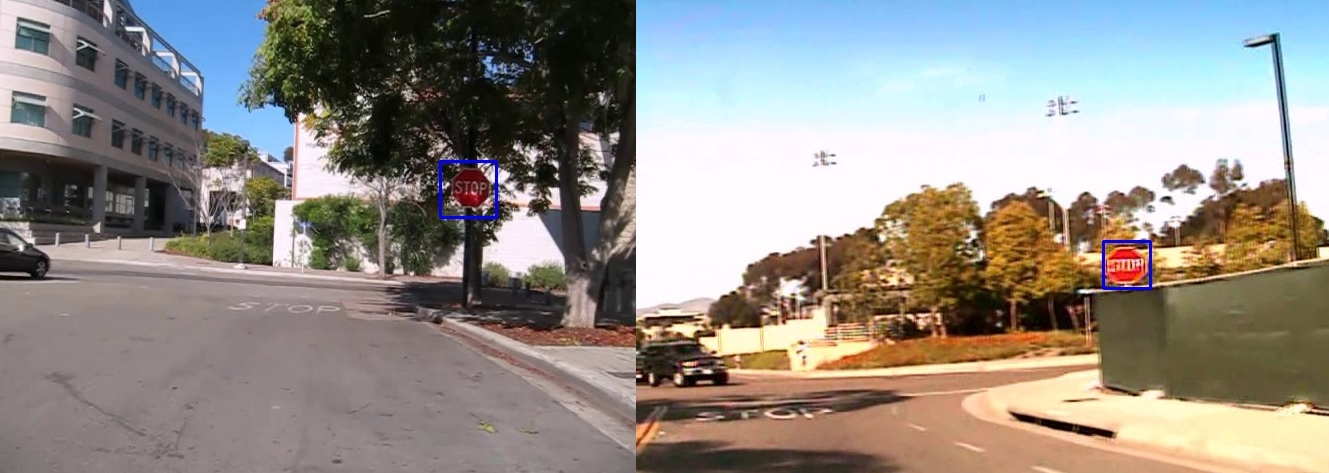
\includegraphics[width=\linewidth]{images/detection.jpg}}
\caption{Stop Sign Detection}
\label{fig:detect}
\end{figure}

After successful testing of stop sign classifier, we proceeded to
train the classifiers for Yield sign and Signal Ahead sign. We trained
3 classifiers each for both these signs while increasing the number of
positive images from 600, 900, 1200. Even after increasing the number
of positive images up to 1200 the resulting classifiers were not
efficient enough to detect the signs in images.  As each training had
resulted in a loss of approximately 3.5 days, we realized that this
could not be covered as part of this project and restricted ourselves
to the stop sign detection.
\subsubsection{Outcomes}
\begin{itemize}
\item From the many experiments we carried out, we learned that there
  is no fixed number of samples that will yield a decent result.
\item Future work can be done on training the U.S traffic signs, since
  there are no classifiers available for them . With the growing
  market for autonomous vehicles and assisted driving technology,
  having trained classifiers for the traffic signs might prove to
  helpful.
\end{itemize}

\section{Execution Summary}
This section specifies the week by week timeline for project
completion.

\begin{enumerate}
\item {Mar 6 - Mar 12, 2017:} During this week we created virtual
  machines on Chameleon cloud using Cloudmesh and submit the project
  proposal.
\item {Mar 13-Mar 19, 2017:} Deployed Hadoop cluster to Chameleon
  cloud using Cloudmesh and develop Ansible playbook to install the
  required software packages to the clusters (OpenCV, Python and
  dependencies)
\item {Mar 20-Mar 26, 2017:} Collated data for training and test data
  sets and trained stop sign classifier. Developed Ansible playbook to
  deploy Hadoop and Spark to the cloud machines.
\item {Mar 27-Apr 02, 2017:} Trained data for stop and yield sign
  classifiers using OpenCV.  Developed Ansible playbook to setup the
  OpenCV python environment on Spark clusters.
\item {Apr 03-Apr 09, 2017:} Trained data for signal ahead sign using
  OpenCV. Test stop sign classifier on local machine and chameleon
  cloud.
\item {Apr 10 - Apr 16, 2017:} Tested classifier on Spark and created
  deployable software package using shell script.
\item {Apr 17-Apr 23, 2017:} Completed project report and developed
  benchmarks for the project.
\end{enumerate}

\end{document}
